\section{Empirical Study}\label{Sec:empirical}
\subsection{Data description: Soichi}
\begin{itemize}
	\item Describe the data and its quality.
	\item How was the data sample selected?
	\item Provide descriptive statistics such as:
	\begin{itemize}
		\item time period,
		\item number of observations, data frequency,
		\item mean, median,
		\item min, max, standard deviation,
		\item skewness, kurtosis, Jarque--Bera statistic,
		\item time series plots, histogram.
	\end{itemize}
	\item For example:
	\begin{table}[ht]
		
		\begin{center}
			{\footnotesize
				\begin{tabular}{l|cccccccccc}
					\hline \hline
					& 3m    & 6m    & 1yr   & 2yr   & 3yr   & 5yr   & 7yr   & 10yr  & 12yr  & 15yr   \\
					\hline
					Mean   & 3.138 & 3.191 & 3.307 & 3.544 & 3.756 & 4.093 & 4.354 & 4.621 & 4.741 & 4.878  \\
					StD    & 0.915 & 0.919 & 0.935 & 0.910 & 0.876 & 0.825 & 0.803 & 0.776 & 0.768 & 0.762  \\
					\hline \hline
				\end{tabular}}
			\end{center}
			\caption{Some descriptive statistics of location and dispersion for
				2100 observed swap rates for the period from February 15, 1999
				to March 2, 2007. Swap rates measured as 3.12 (instead of 0.0312). See Table
				\ref{Tab:DescripStatsRawDataDetail} in the appendix for
				more details.}
			\label{Tab:DescripStatsRawData}
		\end{table}
		
		\item Allows the reader to judge whether the sample is biased or to evaluate possible impacts of outliers, for
		example.
		
	\end{itemize}
\subsection{Regression Specification: Hyerin}
\ \ \ In this section, we discuss the causal effect of income on democracy. The relation between democracy scores and income per capita is estimated using the following simple econometric model:  
\begin{align}
d_{i,t} = \alpha d_{i,t-1} + \gamma y_{i,t-1}+ X'_{i,t-1}\beta + \mu_{t}+\delta_{i} + u_{i,t}
\end{align}
\ \ \ \ The democracy score of coutry $i$ in time period $t$ is denoted by $d_{i,t}$. To capture persistency of it, the lagged value of this variable, $d_{i,t}$, is included as a regressor in the model. $y_{i,t-1}$ denotes the lagged value of country $i$'s log income per capita and the estimated coefficient, $\gamma$, measures the causal effect of income per capita on democracy. If an increase in income per capita leads to an higher score of democracy, then the coefficient on the lagged value of log income per capita $\gamma$ should be positive. A full set of coutry dummies and time effects   $\delta_{i}$ $\mu_{t}$. All other potential covariates are denoted in the vector formation,  $X'_{i,t-1}$. To control for country-specific factors a full set of country dummies, $\delta_{i}$, is included in the right-hand side. In addition, to capture common shocks over all sample countries, it introduces $\mu_{t}$ as a full set of time effects. An error term is denoted as $u_{i,t}$.\\


\subsection{Regression Estimates}
\subsubsection{Fixed Effects: Soichi}
\begin{table}[h!] \centering
			\begin{adjustbox}{max width=\textwidth}
			\begin{threeparttable}
		\caption{\textsc{fixed effects results using freedom house measure of democracy}}
			\begin{tabular}{l*{7}{c}}
         \toprule
			    & \multicolumn{7}{c}{Base sample, 1960-2000}\\
	     \cline{2-8}
	            & & &&& & &Twenty-year\\[-1.8ex]
				& \multicolumn{3}{c}{Five-year data} && \multicolumn{1}{c}{Ten-year data} && \multicolumn{1}{c}{data}\\
		\cline{2-4}\cline{6-6}\cline{8-8}	
		    &Pooled &Fixed effects &Fixed effects &&Fixed effects &&Fixed effects \\[-1.8ex] 	
		    &OLS &OLS &OLS &&OLS &&OLS \\[-1.8ex] 			 
		        &\multicolumn{1}{c}{(1)} &\multicolumn{1}{c}{(2)} &\multicolumn{1}{c}{(3)} &&\multicolumn{1}{c}{(4)} &&\multicolumn{1}{c}{(5)}\\ 
		\hline        
				Democracy$_{t-1}$ & 0.706$^{***}$ & 0.379$^{***}$ &  && -0.025 && -0.581$^{***}$ \\[-1.8ex] 
				 \ & (0.035) & (0.051) &  && (0.088) && (0.198) \\ 
				Log GDP per capita${}_{t-1}$ & 0.072$^{***}$ & 0.010 & 0.054 && 0.053 && -0.030 \\[-1.8ex] 
				 \ & (0.010) & (0.035) & (0.046) && (0.066) && (0.156) \\ 
				Observations & \multicolumn{1}{c}{945} & \multicolumn{1}{c}{945} & \multicolumn{1}{c}{958} && \multicolumn{1}{c}{457} && \multicolumn{1}{c}{192} \\ 
				R${}^{2}$ & \multicolumn{1}{c}{0.725} & \multicolumn{1}{c}{0.242} & \multicolumn{1}{c}{0.118} && \multicolumn{1}{c}{0.122} && \multicolumn{1}{c}{0.452} \\ 
				\hline 
			\end{tabular}
		\begin{tablenotes}
					    	\item \textit{Notes:} 
		\end{tablenotes}
		\end{threeparttable}	
		\end{adjustbox}
	\end{table}

\begin{itemize}
    \item Organize material and present results.
    \item Use tables, figures (but prefer visual presentation):
        \begin{itemize}
            \item Tables and figures should supplement (and not duplicate) the text.
            \item Tables and figures should be provided with legends.\\
                {\it Figure \ref{Fig:Resids} shows how to include and reference
                graphics. The graphic must be labelled before. Files must be in
                \texttt{.eps} format.}

                \begin{figure}[ht]
                \begin{center}
                    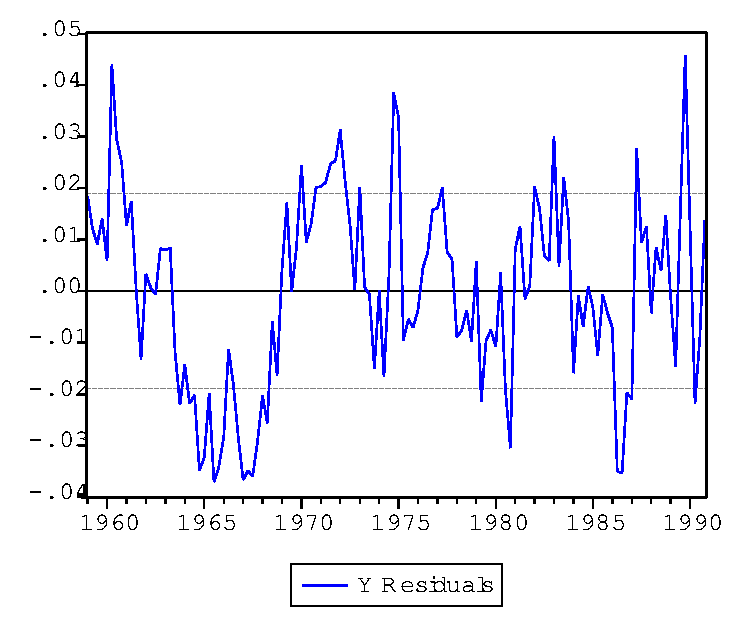
\includegraphics[scale=0.5,angle=0]{graph}
                    \caption{Estimated residuals from model XXX. ...}
                    \label{Fig:Resids}
                \end{center}
                \end{figure}

            \item Tables and graphics may appear in the text or in
                the appendix, especially if there are many simulation results
                tabulated, but is also depends on the study and number of tables resp.
                figures. The key graphs and tables must appear in
                the text!
        \end{itemize}
        

\subsubsection{Instrumental Variable: Hyerin}
In order to estimate the impact of income on democracy identify the causal effect of income on democracy, we need to 
	\begin{table}[h!] 
		\centering
		\begin{adjustbox}{max width=\textwidth}
		\begin{threeparttable}
			\caption{\textsc{fixed effects results using freedom house measure of democracy: Two-stage least squares with savings rate instrument}}			
			\begin{tabular}{l*8{c}}
		    \hline\hline
		    \ &\multicolumn{8}{c}{Base sample, 1960-2000}\\
		    \cline{2-9}
		    \ &\multicolumn{8}{c}{All countries}\\
		    \cline{2-9}
		    &Pooled &Fixed effects &Fixed effects &Fixed effects &Fixed effects &Fixed effects &Fixed effects &Fixed effects\\[-1.8ex] 	
		    &OLS &OLS &OLS &2SLS &2SLS &2SLS &2SLS &2SLS\\[-1.8ex] 
		    &(1) &(2) &(3) &(4) &(5) &(6) &(7) &(8)\\
		    \hline 
			Panel A &\multicolumn{8}{c}{\textit{Dependent variable is democracy}}\\			
			\hline
			Democracy${}_{t-1}$ &  &  & 0.359 &  & 0.363 &  &  &\\[-1.8ex] 
				&  &  &(0.054) &  & (0.056) &  &  &  \\ 
			Log GDP per capita${}_{t-1}$ & 0.233$^{***}$ & 0.044 & 0.009 & -0.035 & -0.020 & -0.036 & -0.074 & 0.016 \\[-1.8ex] 
				& (0.013) & (0.051) & (0.038) & (0.094) & (0.081) & (0.191) & (0.113) & (0.095) \\ 
			Labor share${}_{t-1}$ &  &  &  &  &  & 0.250 &  &  \\[-1.8ex] 
				&  &  &  &  &  & (0.199) &  &  \\
			\hline
			Panel B &\multicolumn{8}{c}{\textit{First stage for log GDP per capita$_{t-1}$}}\\
			\hline			
			Democracy${}_{t-1}$ &  &  &  &  & 0.144$^{**}$ &  & [0.24] &  \\[-1.8ex] 
				&  &  &  &  & (0.066) &  &  &  \\ 
			Labor share${}_{t-1}$ &  &  &  &  &  & 0.329$^{*}$ &  &  \\[-1.8ex] 
				&  &  &  &  &  & (0.187) &  &  \\ 
			Savings rate${}_{t-2}$ &  &  &  & 1.356$^{***}$ & 1.343$^{***}$ & 1.202$^{***}$ & 1.173$^{***}$ & 1.022$^{***}$ \\[-1.8ex] 
				&  &  &  & (0.277) & (0.270) & (0.315) & (0.254) & (0.218) \\ 
			Savings rate${}_{t-3}$ &  &  &  &  &  &  &  & 0.720$^{***}$ \\[-1.8ex] 
				&  &  &  &  &  &  &  & (0.182) \\ 
				Observations &\multicolumn{1}{c}{891} & \multicolumn{1}{c}{900} & \multicolumn{1}{c}{766} & \multicolumn{1}{c}{900} & \multicolumn{1}{c}{891} & \multicolumn{1}{c}{471} & \multicolumn{1}{c}{733} & \multicolumn{1}{c}{796} \\ 
				R$^{2}$ &\multicolumn{1}{c}{0.226} & \multicolumn{1}{c}{0.115} & \multicolumn{1}{c}{0.225} & \multicolumn{1}{c}{0.571} & \multicolumn{1}{c}{0.571} & \multicolumn{1}{c}{0.725} & \multicolumn{1}{c}{0.541} & \multicolumn{1}{c}{0.536} \\ 
				\hline
			\end{tabular}
		    \begin{tablenotes}
		    	\item \textit{Notes:} This table summarizes the codefficients of each cross-sectional regression. All regression model includes year dummies to capture country-invariant factors. Except for column 1, country dummies are included in the regressions. The robust standrad errors clustered by country are summarized in parentheses. 
		    	\item \begin{align}
		    	^{***}& \text{Significant at the 1 percent level}\notag\\
		    	^{**}& \text{Significant at the 5 percent level}\notag\\
		    	^{*}& \text{Significant at the 10 percent level}\notag
		    	\end{align}
		    \end{tablenotes}
		\end{threeparttable}
		\end{adjustbox}			
	\end{table} 	


\newpage
\subsection{Robustness Tests: Sharon}
\textsl{Additional Control Variables.} ---
\\
\textsl{Different Sample Base.} ---
\\
\textsl{Alternative Dependent Variable.} ---
\\
\textsl{Extension of Sample Periods} ---
    \item Discuss results:
        \begin{itemize}
            \item Do the results support or do they contradict economic theory ?
            \item What does the reader learn from the results?
            \item Try to give an intuition for your results.
            \item Provide robustness checks.
            \item Compare to previous research.
        \end{itemize}
\end{itemize}
